\chapter{Feature Engineering}
    Durante il corso della creazione di un modello, è molto probabile (quasi certo) di incontrare problemi con i dati.
    Alcune problematiche che potrebbero sorgere sono, per esempio, la gestione delle features binarie, gestione delle features categoriali o anche dei valori mancanti!
    \\[2\baselineskip]
    Di seguito verranno illustrate alcune strategie per ovviare a questi problemi:
    \begin{itemize}
        \item $\textbf{Features Categoriche Binarie}:$ fare un remapping a 0-1 dei valori (es: Alto $\longrightarrow$ 1; Basso $\longrightarrow$ 0);
        \item $\textbf{Features Categoriche K-arie}:$ One-Hot Encoding (discusso in seguito);
        \item $\textbf{Etichette di Classe Categoriche K-arie}:$ fare un remapping a degli ID numerici;
            \\
            $\textbf{Attebzione:}$ Questa soluzione va bene per i Decision Trees ma non per kNN e Linear Regression!
        \item $\textbf{Features con Valori Singoli}:$ essendo insignificative alla risoluzione di qualsiasi tipo di problema, le si può tranquillamente togliere;
        \item $\textbf{Valori Mancanti}:$ rimpiazzare con la media se è un valore numerico o con la moda se categoriale.
    \end{itemize}

    \subsection{Problemi con i Dati Categoriali}
        Alcuni algoritmi possono funzionare direttamente con i dati categoriali (es: Alberi Decisionali), ma molti altri algoritmi non riescono a processarle e richiedono una trasformazione numerica di queste variabili.

        \subsubsection{Codifica a Numerici Ordinali}
            A ogni valori categorico viene assegnato un valori intero (es: "rosso" $\longrightarrow$ 1, "verde" $\longrightarrow$ 2, "blu" $\longrightarrow$ 3).
            \\[1\baselineskip]
            Bisogna fare attenzione nell'utilizzo di questo metodo perché si va a creare una relazione di ordinamento.
            Questo può essere d'aiuto se si vuole effettivamente rappresentare un ordinamente, ma nelle variabili categoriali in cui non esiste una relazione d'ordine ciò può portare a risultati imprevisti!
            \\
            Prendiamo d'esempio la codifica in valori ordinali del colore degli occhi: dire che "rosso" (1) è tre volte più piccolo di "blu" (3) non ha senso in questo caso.

        \subsubsection{One-Hot Encoding}
            Questo metodo di codifica consiste nella sostituzione della variabile categoriale con $n$ variabili binarie, una per ogni valore che poteva assumere la precedente feature categoriale.
            \begin{figure}[h]
                \caption[short]{Esempio di One-Hot Encoding}
                \centering
                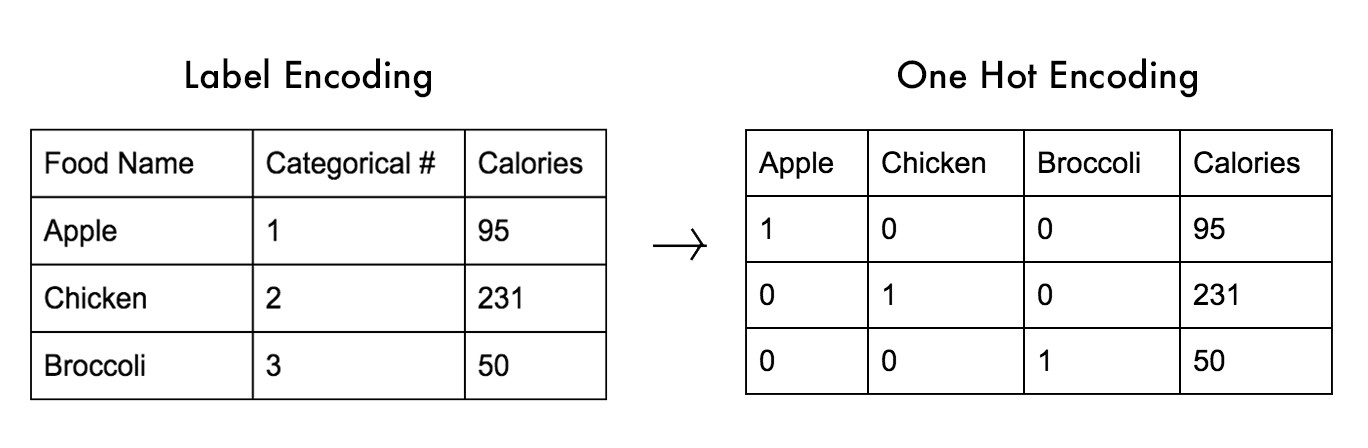
\includegraphics[width = 10cm, height = 2.3cm]{one-hot-example.jpeg}
            \end{figure}
        
    \clearpage